% This template has been tested with LLNCS DOCUMENT CLASS -- version 2.20 (24-JUN-2015)

%"runningheads" enables:
%  - page number on page 2 onwards
%  - title/authors on even/odd pages
%This is good for other readers to enable proper archiving among other papers and pointing to
%content. Even if the title page states the title, when printed and stored in a folder, when
%blindly opening the folder, one could hit not the title page, but an arbitrary page. Therefore,
%it is good to have title printed on the pages, too.
\documentclass[runningheads,a4paper]{llncs}[2015/06/24]

%cmap has to be loaded before any font package (such as cfr-lm)
\usepackage{cmap}
\usepackage[T1]{fontenc}

%https://tex.stackexchange.com/questions/57743/how-to-write-%c3%a4-and-other-umlauts-and-accented-letters-in-bibliography#57745
%for german umlauts
\usepackage[utf8]{inputenc}

\usepackage{graphicx}

%Even though `american`, `english` and `USenglish` are synonyms for babel package (according to https://tex.stackexchange.com/questions/12775/babel-english-american-usenglish), the llncs document class is prepared to avoid the overriding of certain names (such as "Abstract." -> "Abstract" or "Fig." -> "Figure") when using `english`, but not when using the other 2.
%english has to go last to set it as default language
\usepackage[ngerman,english]{babel}
%Hint by http://tex.stackexchange.com/a/321066/9075 -> enable "= as dashes
\addto\extrasenglish{\languageshorthands{ngerman}\useshorthands{"}}

%better font, similar to the default springer font
%cfr-lm is preferred over lmodern. Reasoning at http://tex.stackexchange.com/a/247543/9075
\usepackage[%
rm={oldstyle=false,proportional=true},%
sf={oldstyle=false,proportional=true},%
tt={oldstyle=false,proportional=true,variable=true},%
qt=false%
]{cfr-lm}
%
%if more space is needed, exchange cfr-lm by mathptmx
%\usepackage{mathptmx}

%for demonstration purposes only
\usepackage[math]{blindtext}

%Sorts the citations in the brackets
%It also allows \cite{refa, refb}. Otherwise, the document does not compile.
%  Error message: "White space in argument"
\usepackage{cite}


%% If you need packages for other papers,
%% START COPYING HERE
%% COPY ALSO cmap and fontenc from lines 10 to 12

%extended enumerate, such as \begin{compactenum}
\usepackage{paralist}

%put figures inside a text
%\usepackage{picins}
%use
%\piccaptioninside
%\piccaption{...}
%\parpic[r]{\includegraphics ...}
%Text...

%for easy quotations: \enquote{text}
\usepackage{csquotes}

%enable margin kerning
\usepackage{microtype}

%tweak \url{...}
\usepackage{url}
%\urlstyle{same}
%improve wrapping of URLs - hint by http://tex.stackexchange.com/a/10419/9075
\makeatletter
\g@addto@macro{\UrlBreaks}{\UrlOrds}
\makeatother
%nicer // - solution by http://tex.stackexchange.com/a/98470/9075
%DO NOT ACTIVATE -> prevents line breaks
%\makeatletter
%\def\Url@twoslashes{\mathchar`\/\@ifnextchar/{\kern-.2em}{}}
%\g@addto@macro\UrlSpecials{\do\/{\Url@twoslashes}}
%\makeatother

%diagonal lines in a table - http://tex.stackexchange.com/questions/17745/diagonal-lines-in-table-cell
%slashbox is not available in texlive (due to licensing) and also gives bad results. This, we use diagbox
%\usepackage{diagbox}

%required for pdfcomment later
\usepackage{xcolor}


%enable nice comments
%this also loads hyperref
\usepackage{pdfcomment}
%enable hyperref without colors and without bookmarks
\hypersetup{hidelinks,
   colorlinks=true,
   allcolors=black,
   pdfstartview=Fit,
   breaklinks=true}
%enables correct jumping to figures when referencing
\usepackage[all]{hypcap}

\newcommand{\commentontext}[2]{\colorbox{yellow!60}{#1}\pdfcomment[color={0.234 0.867 0.211},hoffset=-6pt,voffset=10pt,opacity=0.5]{#2}}
\newcommand{\commentatside}[1]{\pdfcomment[color={0.045 0.278 0.643},icon=Note]{#1}}

%compatibality with packages todo, easy-todo, todonotes
\newcommand{\todo}[1]{\commentatside{#1}}
%compatiblity with package fixmetodonotes
\newcommand{\TODO}[1]{\commentatside{#1}}

%enable \cref{...} and \Cref{...} instead of \ref: Type of reference included in the link
\usepackage[capitalise,nameinlink]{cleveref}
%Nice formats for \cref
\crefname{section}{Sect.}{Sect.}
\Crefname{section}{Section}{Sections}

\usepackage{xspace}
%\newcommand{\eg}{e.\,g.\xspace}
%\newcommand{\ie}{i.\,e.\xspace}
\newcommand{\eg}{e.\,g.,\ }
\newcommand{\ie}{i.\,e.,\ }

%introduce \powerset - hint by http://matheplanet.com/matheplanet/nuke/html/viewtopic.php?topic=136492&post_id=997377
\DeclareFontFamily{U}{MnSymbolC}{}
\DeclareSymbolFont{MnSyC}{U}{MnSymbolC}{m}{n}
\DeclareFontShape{U}{MnSymbolC}{m}{n}{
    <-6>  MnSymbolC5
   <6-7>  MnSymbolC6
   <7-8>  MnSymbolC7
   <8-9>  MnSymbolC8
   <9-10> MnSymbolC9
  <10-12> MnSymbolC10
  <12->   MnSymbolC12%
}{}
\DeclareMathSymbol{\powerset}{\mathord}{MnSyC}{180}

% correct bad hyphenation here
\hyphenation{op-tical net-works semi-conduc-tor}

%% END COPYING HERE


\begin{document}

\title{Bilderkennung mit Convolutional Neural Networks}
%If Title is too long, use \titlerunning
%\titlerunning{Short Title}

%Single insitute
\author{Ivo Tremel \and Lennard Nöhren}
%If there are too many authors, use \authorrunning
%\authorrunning{First Author et al.}
\institute{Computational Health Informatics}

%Multiple insitutes
%Currently disabled
%
\iffalse
%Multiple institutes are typeset as follows:
\author{Firstname Lastname\inst{1} \and Firstname Lastname\inst{2} }
%If there are too many authors, use \authorrunning
%\authorrunning{First Author et al.}

\institute{
Insitute 1\\
\email{...}\and
Insitute 2\\
\email{...}
}
\fi
			
\maketitle

\begin{abstract}
Wir haben ein aufs Wesentliches reduziertes Faltungsnetz zur Klassifizierung von je 100  verschiedenen, handschriftlichen Buchstaben
in zehn verschiedene Kategorien trainiert. Dabei wurde eine Genauigkeit von 70\% erreicht. Das convolutional neural network (CNN) besteht aus einer Faltungsebene, die von einer Max-Pooling Ebene und einer Fully-Connected Ebene gefolgt wird. Zudem wurde die Erweiterung der Inception-Layers verwendet.
\end{abstract}

\begin{keywords}
keyword1, keyword2
\end{keywords}

%%%%%%%%%%%%%%%%%%%%%%%%%%%%%%%%%%%%%%%%%%%%%%%%%%%%%%%%%%%%%%%%%%%%%%%%%%%%%%%
\section{Introduction}\label{sec:intro}
%%%%%%%%%%%%%%%%%%%%%%%%%%%%%%%%%%%%%%%%%%%%%%%%%%%%%%%%%%%%%%%%%%%%%%%%%%%%%%%

Convolutional Neural Networks kommen nahe an menschliche Leistungen heran und der Ansatz der Faltungsnetze bewahrt die entscheidende Lokalität der Bildinformationen. Allerdings


%\blindtext\todo{Refine me}

Winery~\cite{Winery} is graphical \commentontext{modeling}{modeling with one \enquote{l}, because of AE} tool.

\begin{figure}
Simple Figure
\caption{Simple Figure}
\label{fig:simple}
\end{figure}

\begin{table}
\caption{Simple Table}

\label{tab:simple}
Simple Table
\end{table}

cref Demonstration: Cref at beginning of sentence, cref in all other cases.

\Cref{fig:simple} shows a simple fact, although \cref{fig:simple} could also show something else.

\Cref{tab:simple} shows a simple fact, although \cref{tab:simple} could also show something else.

\Cref{sec:intro} shows a simple fact, although \cref{sec:intro} could also show something else.

Brackets work as designed:
<test>

The symbol for powerset is now correct: $\powerset$ and not a Weierstrass p ($\wp$).

\begin{inparaenum}
\item All these items...
\item ...appear in one line
\item This is enabled by the paralist package.
\end{inparaenum}

``something in quotes'' using plain tex or use \enquote{the enquote command}.

You can now write words containing hyphens which are hyphenated (application"=specific) at other places.
This is enabled by an additional configuration of the babel package.
In case you write \enquote{application-specific}, then the word will only be hyphenated at the dash.
You can also write applica\allowbreak{}tion-specific, but this is much more effort.

\section{Materials and Methods}\label{sec:material}
\subsubsection*{Convolutional Layers}

\subsubsection*{Pooling Layers}
In CNNs fassen Pooling-Layers den Output von den vorhergehenden Neuronen entsprechend der gewählten Kernelgröße zusammen. Dabei wird bei einem 2x2 Kernel der größte Output durchgeschaltet und die anderen drei Ausgänge verworfen. Damit wird eine Reduktion der Datenmenge erreicht, die eine insgesamt schnellere Berechnung ermöglicht.
\subsubsection*{Architektur}
\begin{figure}
	\caption{Main Graph}
	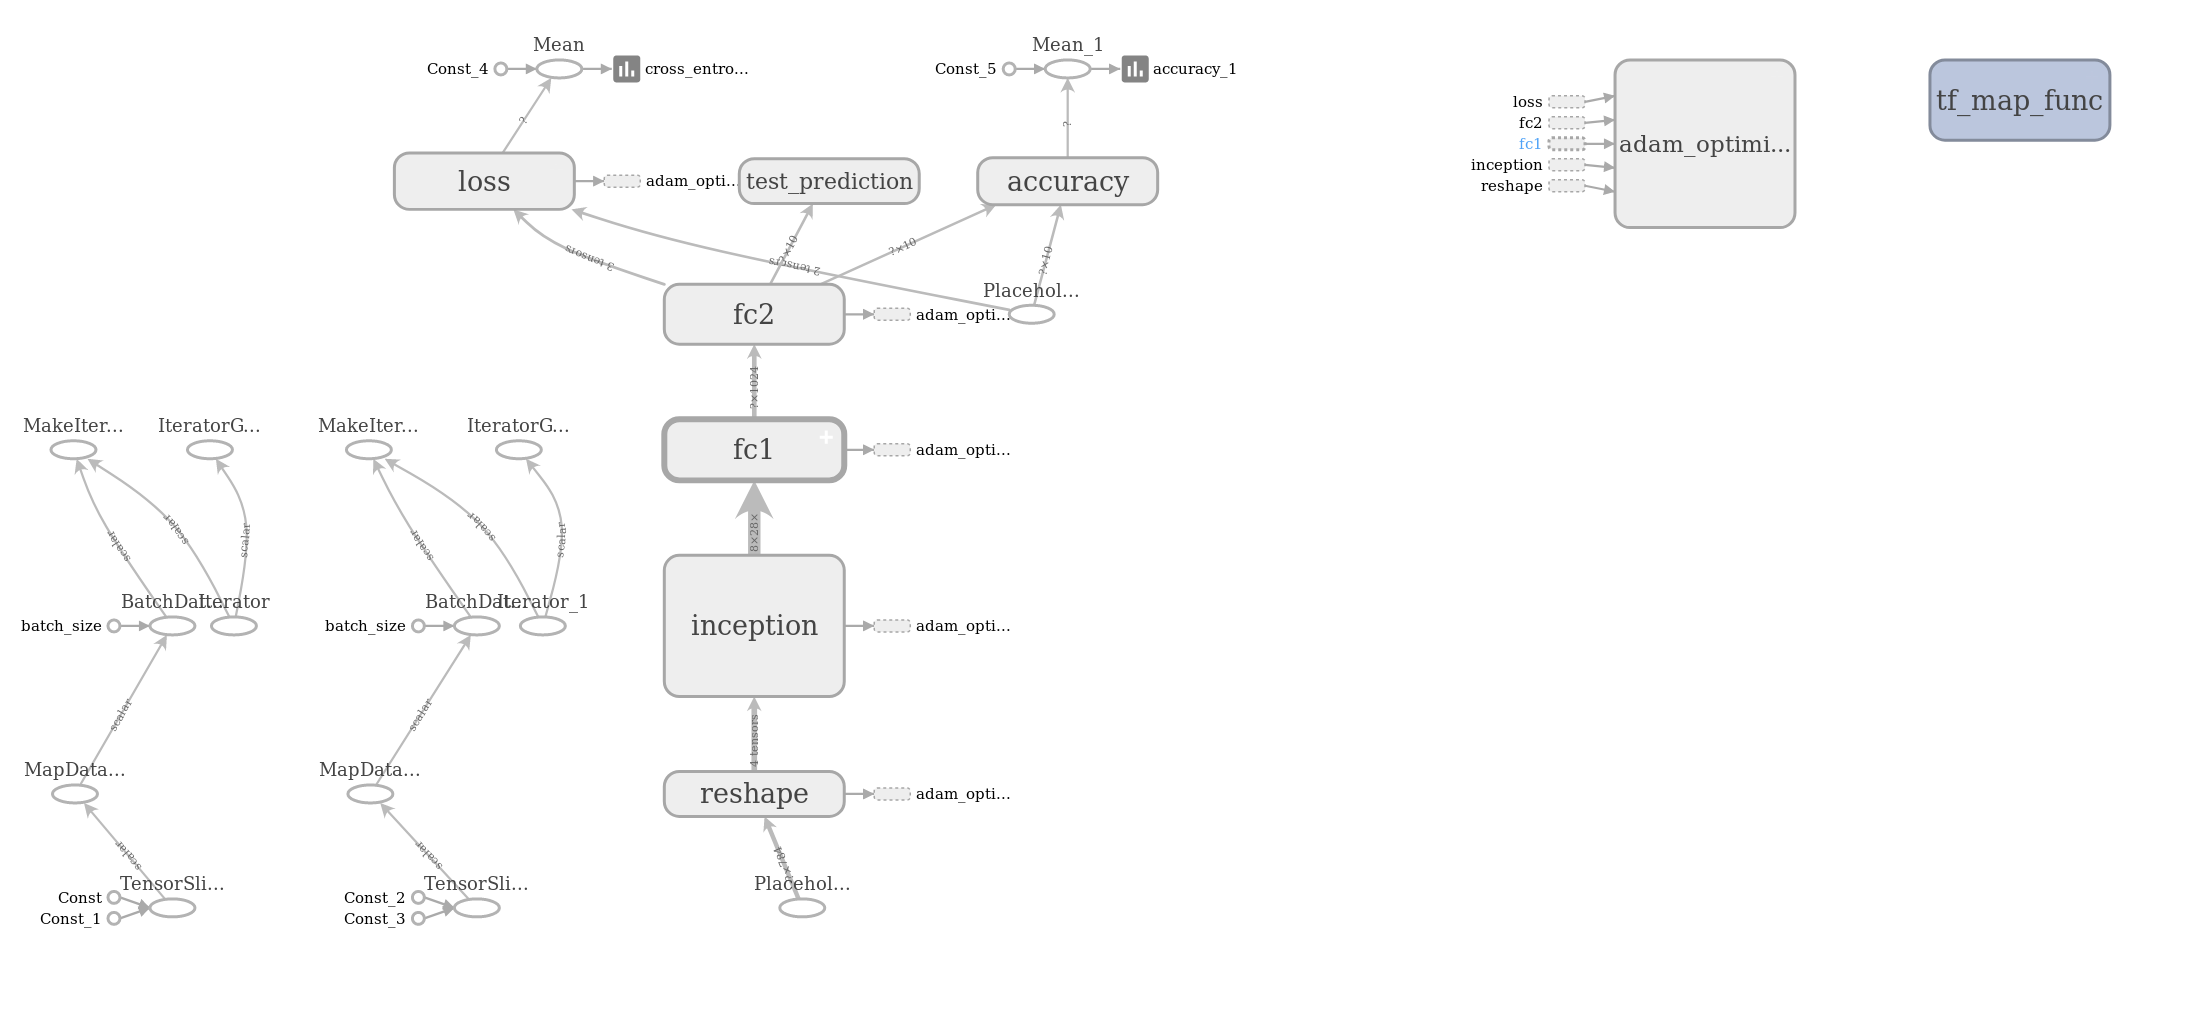
\includegraphics[width=\textwidth]{images/main_graph.png}
	\label{fig:main_graph}
\end{figure}\Cref{fig:main_graph} zeigt den Aufbau des CNNs. Vor dem ersten convolutional Layer wird das Eingabebild zu einem 28x28x1 Bild transformiert. Die erste und zweite Dimension stehen dabei für die Bildhöhe und Bildbreite. Die dritte Dimension bezeichnet die Anzahl von Farbkanälen. Da es sich um ein Graustufenbild handelt und nicht RGB wird der Wert 1 angenommen. 
Bei der convolution werden mit einer Kernelgröße von 5x5 32 features erzeugt.


\section{Results}\label{sec:result}
\section{Discussion}\label{sec:Discussion}

\section{Conclusion and Outlook}
Unsere Ergebnisse zeigen, dass das zusätzliche Convolution-Layer eine weiter Verbesserung bei der Image Klassifizierung bringt.
\subsubsection*{Acknowledgments}
...

In the bibliography, use \texttt{\textbackslash textsuperscript} for ``st'', ``nd'', ...:
E.g., \enquote{The 2\textsuperscript{nd} conference on examples}.
When you use \href{https://www.jabref.org}{JabRef}, you can use the clean up command to achieve that.
See \url{https://help.jabref.org/en/CleanupEntries} for an overview of the cleanup functionality.

%%%%%%%%%%%%%%%%%%%%%%%%%%%%%%%%%%%%%%%%%%%%%%%%%%%%%%%%%%%%%%%%%%%%%%%%%%%%%%%
\bibliographystyle{splncs03}
\bibliography{paper}

All links were last followed on October 5, 2014.
%%%%%%%%%%%%%%%%%%%%%%%%%%%%%%%%%%%%%%%%%%%%%%%%%%%%%%%%%%%%%%%%%%%%%%%%%%%%%%%

\end{document}
